\recipe{Lucy's Veggie Spag Bol}
\label{recipe:veggie_spag_bol}
\makes{5? portions}
\worktime{\SI{30} \minute}
\totaltime{\SI{30} \minute}
\source{Lucy}


\begin{ingredients}

  \item 1 small White Onion, diced
  \item \SI{130}{\gram}  Carrot, finely diced
  \item \SI{100}{\gram} Celery, finely diced
  \item \qty{0.33}{\cup} Dry White Wine + the rest of the bottle for chef .

  \item \SI{200}{\gram} Baby Mushrooms, roughly diced
  \item \SI{300}{\gram} Dry Green Lentils - I use the dried green lentils and part cook them (about \SI{15}{\minute}) so they still have a bit of bite and set aside to add with the other ingredients. 
Alternatively tinned but bolognese will have less texture.
  \item A good dollop of marmite in \SI{500}{\milli \litre} boiling water 
  \item  2 1/2 tins Crushed Tomatoes
  \item \SI{0.33}{\cup} Parsley, finely chopped
  \item 5 large Basil leaves, chopped
  \item 2 Bay Leaves
  \item  \qty{0.5}{\cup} Walnuts, roughly chopped
  \item Cooked Pasta
\end{ingredients}


\begin{method}
Add the Onion, Celery, and Carrot to a large nonstick pot with a
splash of water. Sauté over Medium-High heat until translucent (4
5minutes).

Once all of the water has evaporated from the pan, deglaze with
White Wine; sauté for another 5 minutes

When the pot is dry again, add the Mushrooms, (part cooked) Lentils,
Crushed Tomatoes, Marmite mix, and a splash of water (you can add
more water later if needed); stir well and simmer over high heat.

Once simmering, add the Bay Leaves, Parsley, and Basil. Stir into the
Bolognese and let the whole mixture simmer for 20 minutes or until the
Lentils are tender. Reduce the heat as you go and stir occasionally so
nothing sticks to the bottom.

Note: If there is still too much liquid, drain off any excess and fast
boil in a separate small pan to reduce and add back in

Stir in the chopped Walnuts, and add Salt and Black Pepper. Serve
over cooked pasta.

\end{method}


\begin{figure}[h]
  	\centering
  	
  	\begin{tikzpicture}
  		% Save the image in a box to get its dimensions
  		\sbox0{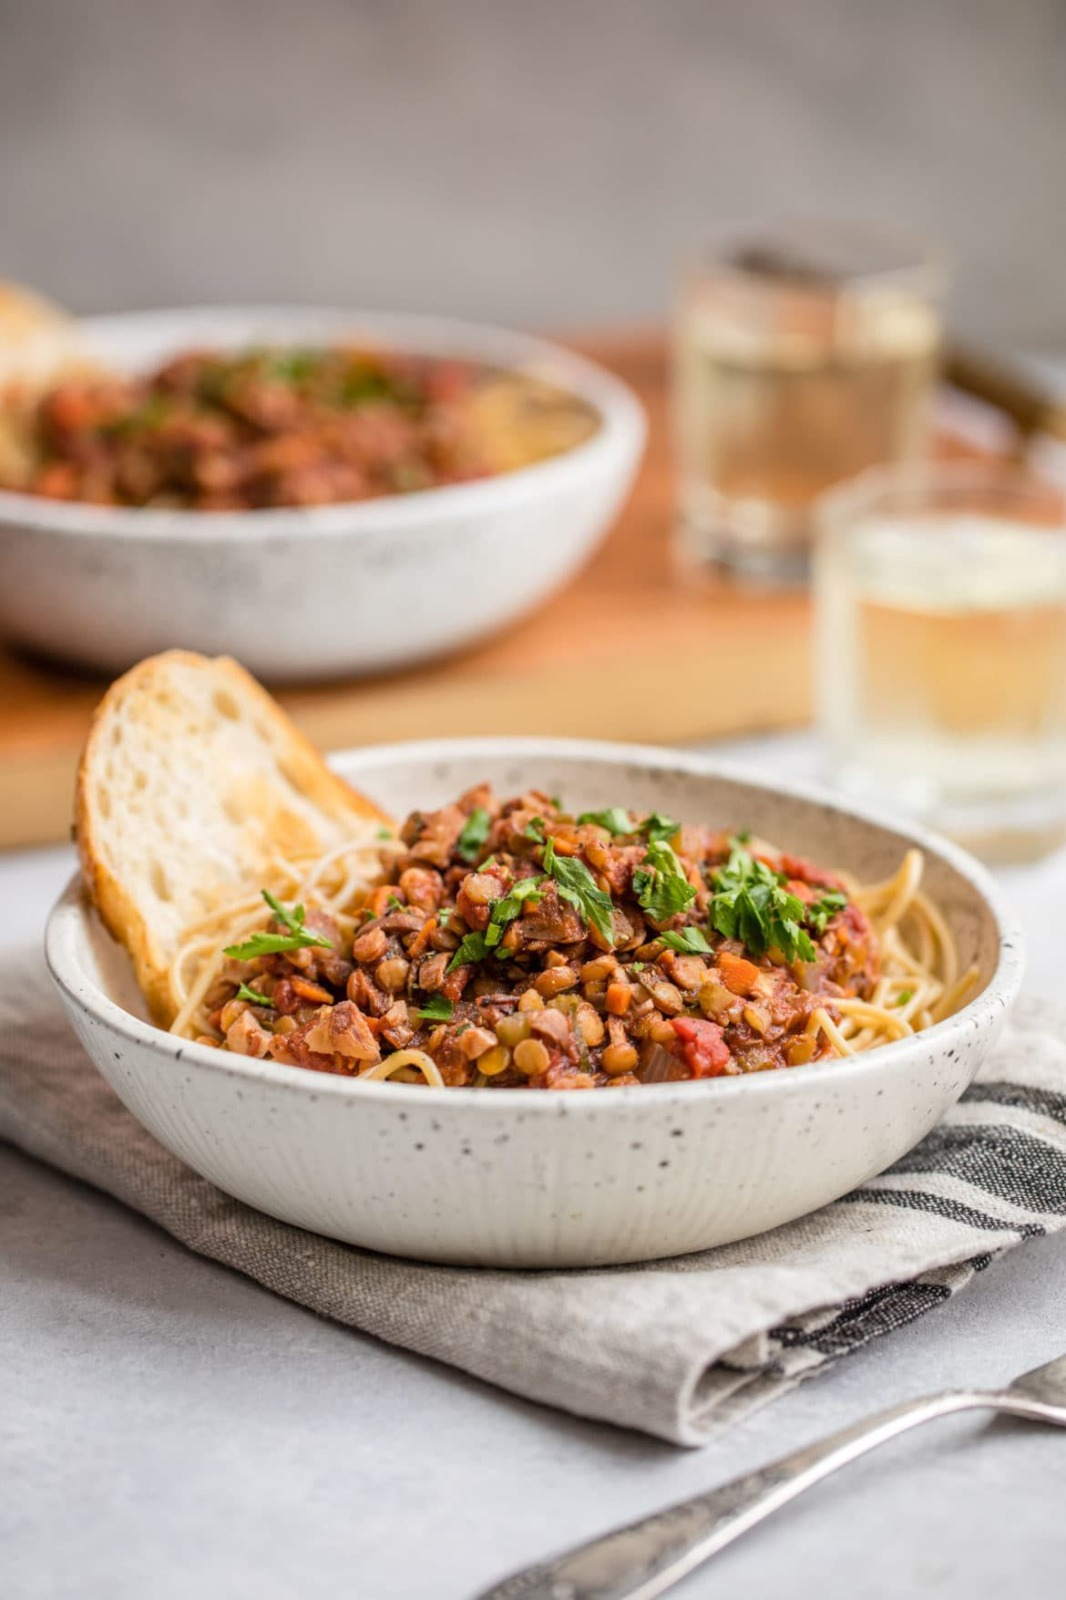
\includegraphics[width = 0.2\linewidth]{images/veggieSpagBol.jpeg}}%
  
  		% Draw a clipping rectangle with rounded corners
  		\path[clip, rounded corners=0.5cm] (0,0) rectangle (\wd0,\ht0);
  
  		% Place the image inside the clipped area
  		\node[inner sep=0pt, outer sep=0pt, anchor=south west] at (0,0) {\usebox0};
	\end{tikzpicture}

  \caption*{}
\end{figure}

\begin{notes}
Leftovers last in the fridge for a week and in the freezer for a month
\end{notes}

